%!TEX root = ../../super_main.tex

\section{The Campaign Model}
Conceptually, a \emph{snapshots} is a snippet of the reality (context) that a specific participants exists in, measured through the subjects devices along with a \emph{label}, describing this reality further. This label is used to define the reality in ways that available sensors cannot. By examining snapshots, and their labels, customers will be able to recognize patterns in measurements, and be able to see a correlation between sensor output and human dynamics. To see development of patterns in time, multiple measurements might be required. To facilitate this, a snapshot consists of a series of \emph{measurements}, each divided into \emph{samples}. To avoid collection redundant data, and wasting the participants resources, the customer must specify what sensors are required, the temporal properties of snapshots, and also how the data should be labeled. This is done through specifying a \emph{campaign}, which participants can contribute to. 
\\\\
One could imagine that a customer might be interested in finding a correlation between heart rate and movement patterns and the influence of alcohol. To do this, a customer would specify a campaign, which should collect information regarding sensors such as \emph{heart rate}, \emph{accelerometer}, and \emph{GPS location}. To know if the participants have consumed alcohol, the customer would specify that participants should indicate if they are, or have been, under the influence of alcohol at a specific time. When contributing information to this campaign, participants would submit snapshots matching this specification. An illustration of how these snapshots are structured can be seen in \figref{fig:snapshot_example}. In this example, the participants are asked to label the snapshot by answering the question \emph{Are you under the influence by alcohol?}.

\begin{figure}[!htbp]
    \centering
    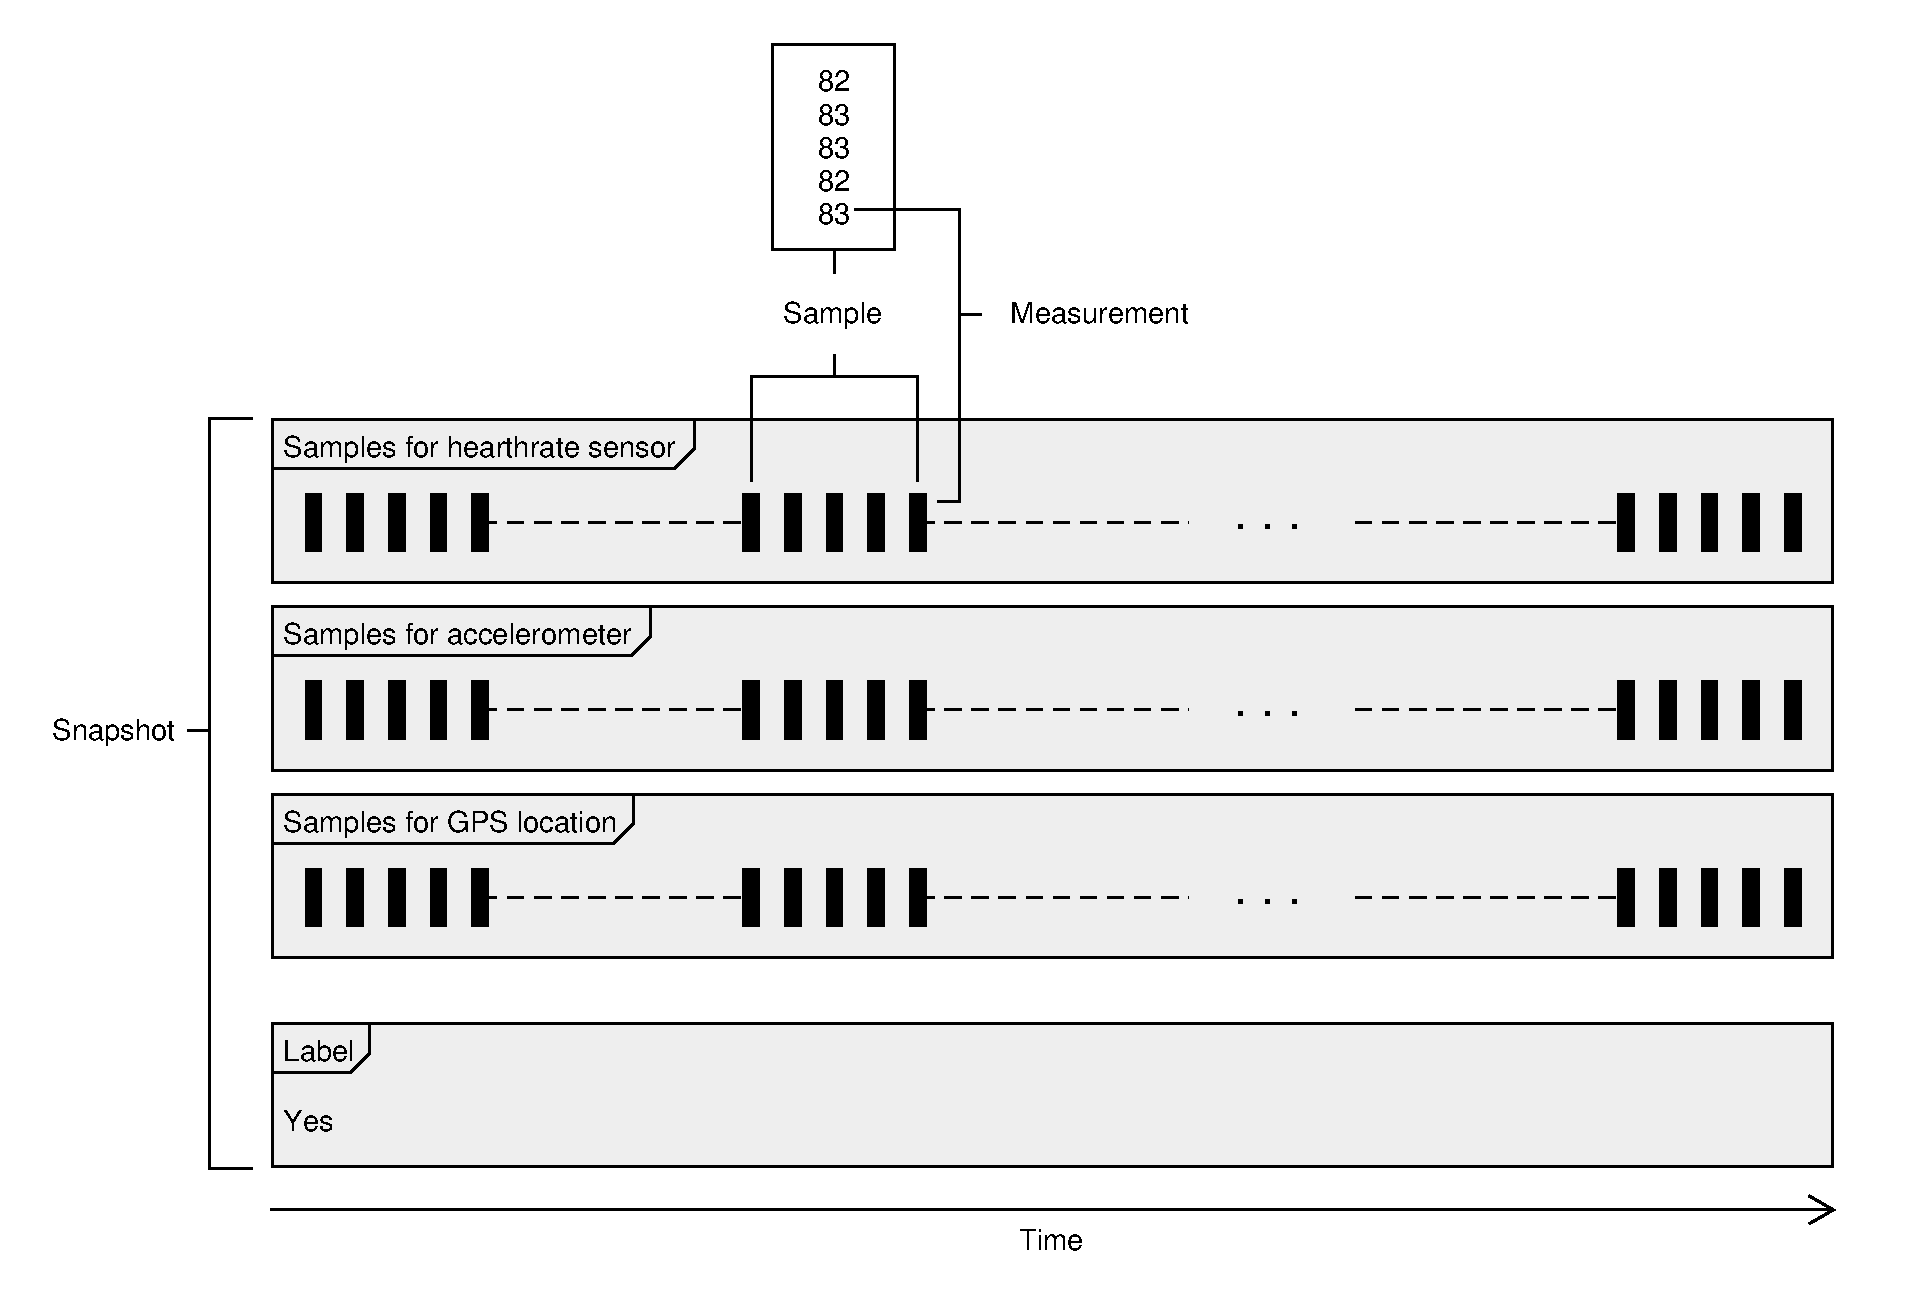
\includegraphics[width=\textwidth]{gathering_sensor_data/snapshot}
    \caption{Snapshot example containing measurements from three sensors and a label.}
    \label{fig:snapshot_example}
\end{figure}
\FloatBarrier

%!TEX root = ../../super_main.tex
\section{Structural Sensor Data}
\label{sec:structural_sensor_data}

Ideally we want to give the customers the ability to configure their campaigns completely in regards to what, i.e. which sensors should be included, and when the outputs from the sensors should be measured. This should be done in such a way that the customers can specify what data is important to them and still avoid draining the resources of the participants devices. For this reason we have designed a way to provide customers with the possibility to configure the temporality of their snapshots. 
\\\\
We go under the assumption that it will be possible to eaves drop in at all times meaning that we can retrieve a measurement from any sensor at all times, however this is not the case but this assumption is enforced as described in \secref{sec:providing_sensor_data}. With the axiom of the sensors we have structured the data from the sensors to be collected as shown in \figref{fig:sample_temporality}. In this figure we see the \emph{measurement} which corresponds to one reading or value of a sensor in a snapshot. Since a single \emph{measurement} from a continuous sensors does not make sense on their own, for instance a single measurement from accelerometer does describe the context in which the participants exist. We introduce a collection of such measurements which we call a \emph{sample}. A \emph{sample} is simply a stream of \emph{measurement}s where the interval or frequency (\emph{measurement frequency}) between them is configurable as seen in \figref{fig:sample_temporality}.

\begin{figure}[!htbp]
    \centering
    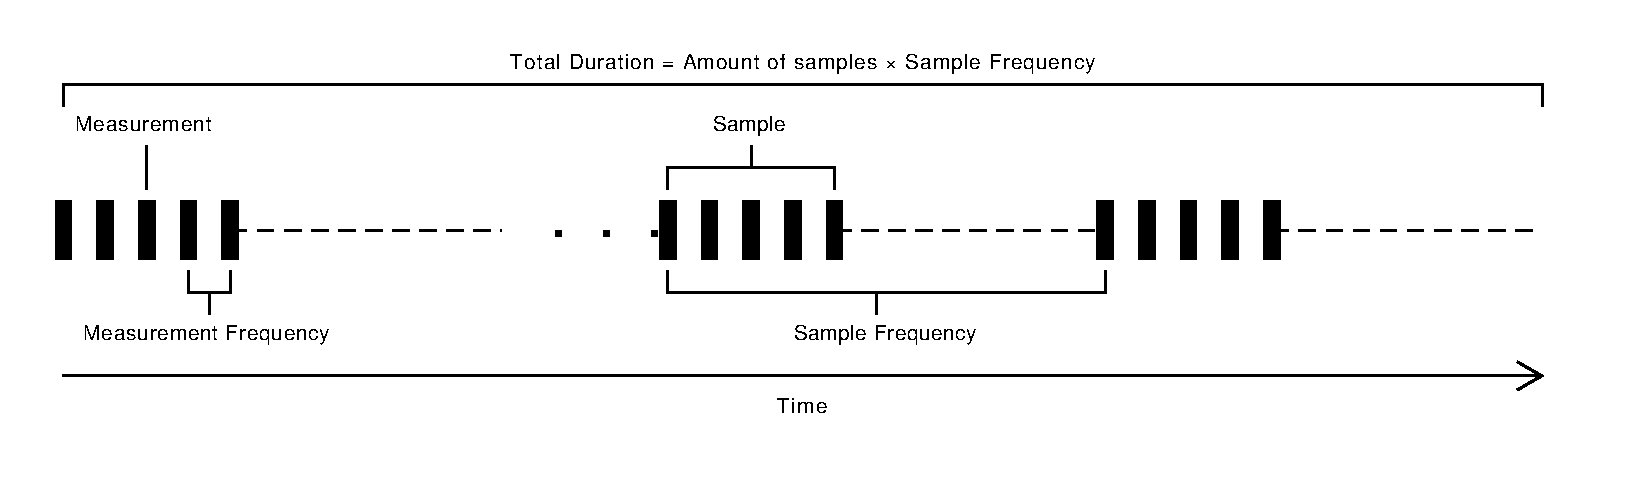
\includegraphics[width=\textwidth]{gathering_sensor_data/sample_temporality.pdf}
    \caption{Temporality of data for a single sensor in a snapshot.}
    \label{fig:sample_temporality}
\end{figure}
\FloatBarrier

Furthermore, we want the customer to configure how often these \emph{sample}s should be gathered, and for that reason we allow them to define a \emph{sample frequency}. And lastly the length of the of the snapshots is configurable by defining a \emph{total duration}, which states for how long the sensor should be measured in total.
\\\\
By this temporal structure of the sensor data we provide a viable way of configuring how the snapshots should be structured in regards to the sensor readings, while maintaining a uniform output format for customers of the system.

\todo[inline]{Vi har reelt 3 forskellige tider: Hvor længe skal et sample vare, hvor ofte skal vi tage et sample, hvor længe skal der gå imellem measurements i et sample? På grund af at sensore i Android giver svar når de har lyst, er det ikke sikkert at der kommer den samme mængde measurements i hver sample. Vi skal overveje om det giver mening, eller om det er vigtigere for kunden at hvert sample med garenti indeholder x measures. Problemet med dette er så at vi ikke kan sætte nogen garenti for hvornår disse measures reelt kommer.}
